\section{Auswertung}
\label{sec:Auswertung}

%Siehe \autoref{fig:plot}!
\subsection{gedämpfte Schwingung}
\label{sec:gedaempft}
Die gemessen Werte für die Spannung am Kondensator $U_\text{C}$ bei Frequenz $f$ sind in der Tabelle \ref{tab:gedaempft} aufgetragen.
Die Schwingung ist in Abbildung \ref{fig:schwingung} zu sehen.
In der Abbildung \ref{fig:ausgleich} sind die Messwerte halblogarythmisch aufgetragen.
Außerdem wurde durch die Funktion 
\begin{equation}
    A = A_0 \symup{e}^{-2 \pi \mu t}
\end{equation}
eine Ausgleichsrechung durchgeführt, dessen Graph ebenfalls in \ref{fig:ausgleich} zu finden ist.
Die Ausgleichsrechung hat folgende Werte ergeben
\begin{equation*}
    A_0 = \SI{1.7004}{}
\end{equation*}
\begin{equation*}
    \mu = \SI{642.3597}{}.
\end{equation*}
Aus den Werten der Ausgleichrechung folgt mit \eqref{eqn:mu} und \eqref{eqn:T}
\begin{equation*}
    T_0 = \SI{0.2477}{\milli\second}.
\end{equation*}
\begin{equation*}
    R_\text{eff} = \SI{136.1768(4036)}{\ohm}
\end{equation*}

%Tabelle mit den Messwerten zur gedämpften Schwingung, 
%gemessen wurde dabei die Spannung in Abhängigkeit von der Zeit
\begin{table}
\centering
\caption{Die Spannungswerte zu verschiedenen Zeitpunkten während einer gedämpften Schwingung.}
\begin{tabular}[t]{cc}
    \toprule
    $t \, / \, \si{\milli\s}$ & $U \,/\, \si{\milli\V}$ \\
    \midrule
    0.000&-125\\
    0.025&135\\
    0.045&-110\\    
    0.060&110\\
    0.075&-95\\
    0.095&95\\
    0.115&-90\\
    0.135&80\\
    0.150&-75\\
    0.170&70\\
    0.190&-65\\
    0.210&60\\
\end{tabular}
\begin{tabular}[t]{cc}
    \toprule
    $t \, / \, \si{\milli\s}$ & $U \,/\, \si{\milli\V}$ \\
    \midrule
    0.225&-55\\
    0.245&50\\
    0.260&-45\\
    0.280&45\\
    0.300&-40\\
    0.320&35\\
    0.335&-35\\
    0.355&30\\
    0.370&-30\\
    0.390&25\\
    0.410&-25\\
    \bottomrule
\end{tabular}
\label{tab:gedaempft}
\end{table}

\begin{figure}
\centering
\caption{Die gedämpfte Schwingung.}
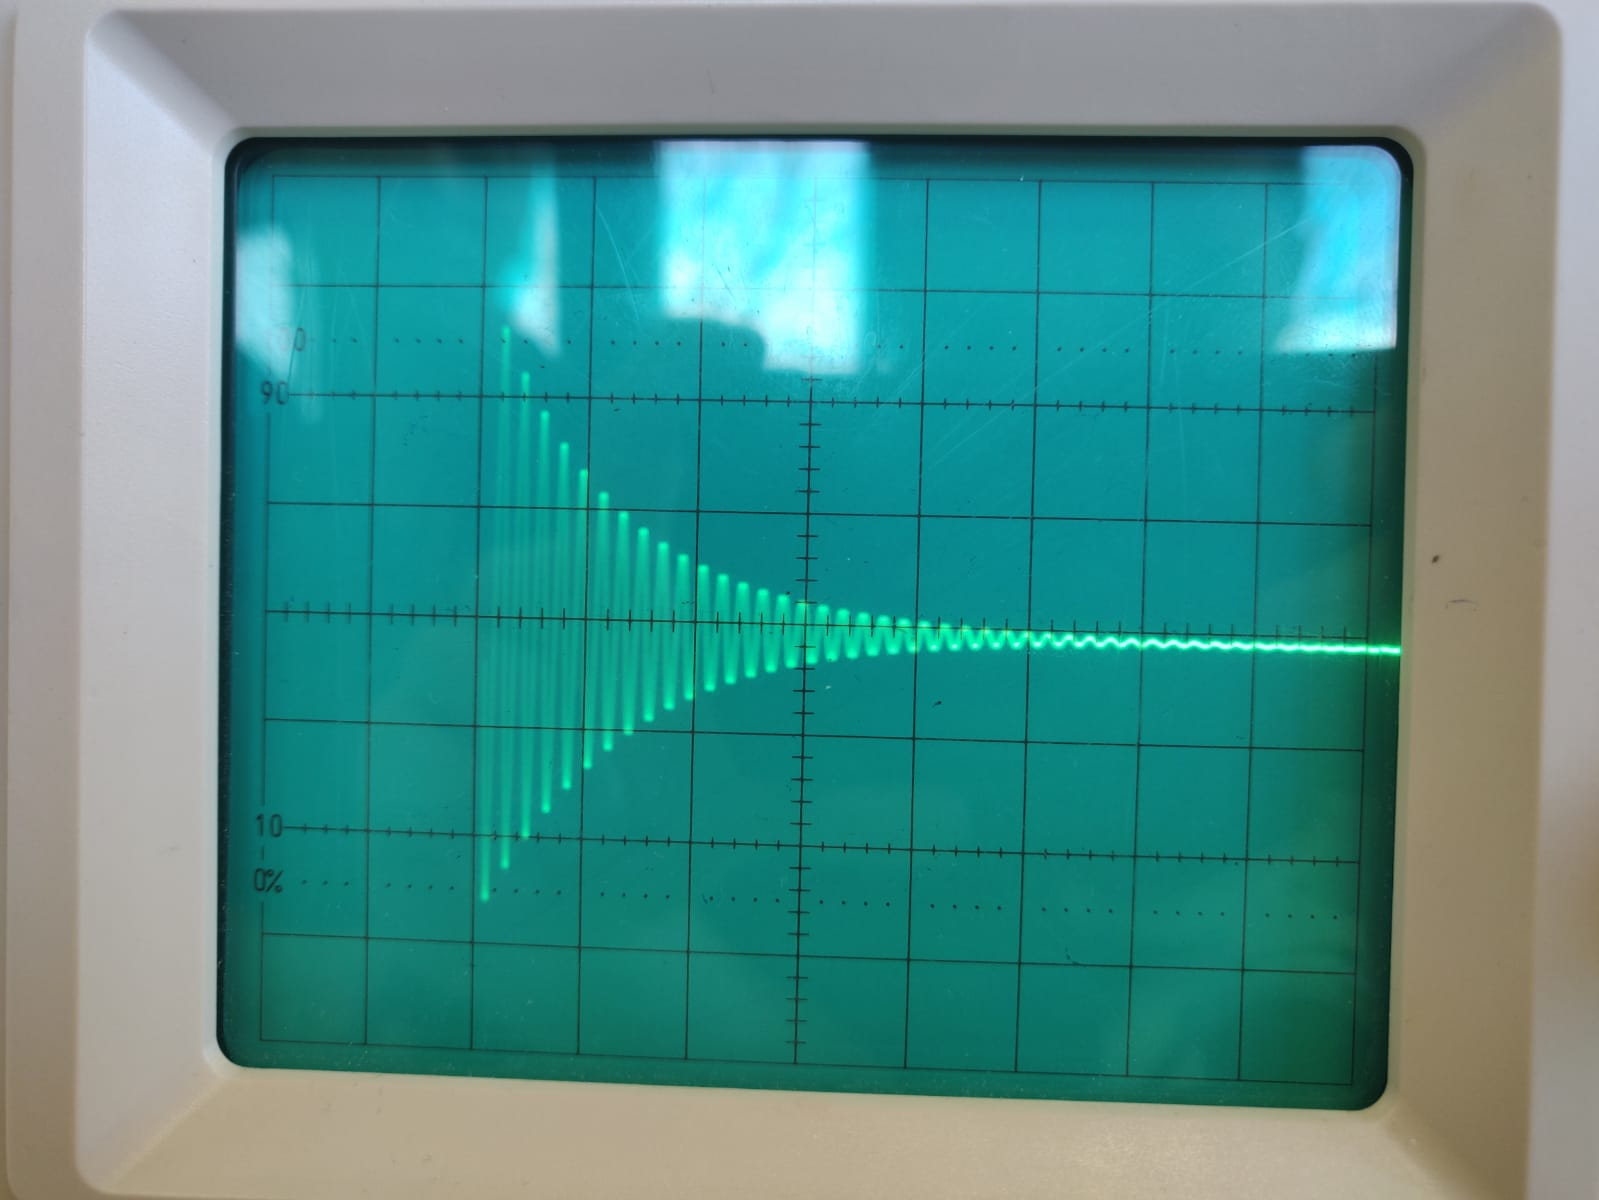
\includegraphics[width=\textwidth]{content/data/schwingung_gedaempft.jpeg}
\label{fig:schwingung}
\end{figure}


\begin{figure}
\centering
\caption{Die Messwerte mit Ausgleichsrechung, die Ausgleichrechnung wurde mit \cite{matplotlib} durchgeführt.}
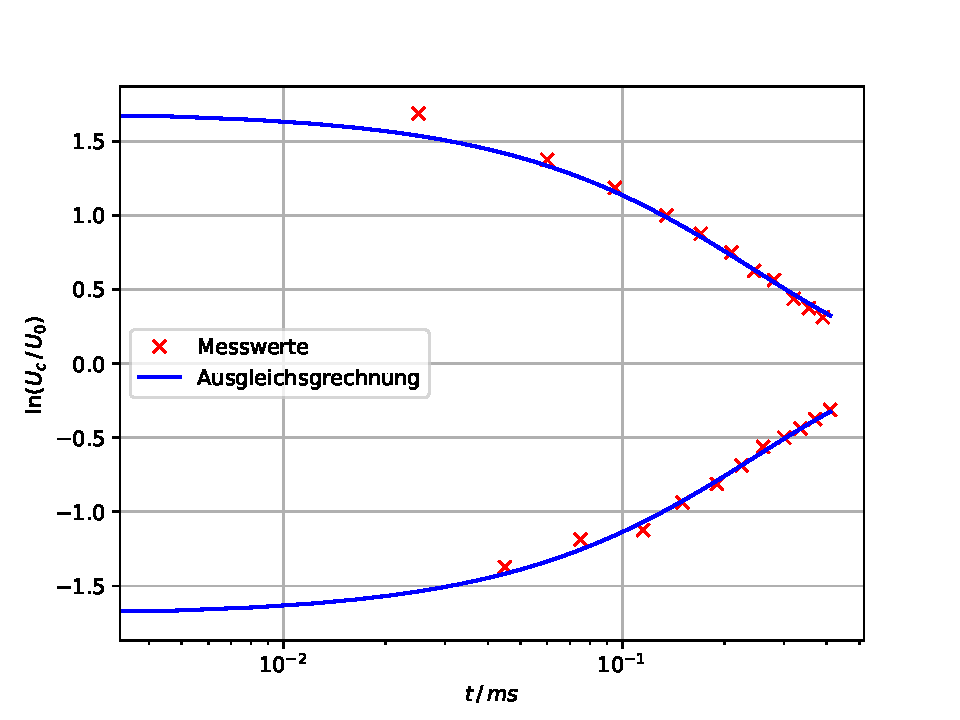
\includegraphics[width=\textwidth]{content/data/plota.pdf}
\label{fig:ausgleich}
\end{figure}

\FloatBarrier

\subsection{aperiodischer Grenzfall}
%U_0/mV, R_p/kOhm
%180, 5
Zu einer Spannung von $U_0 = \SI{180}{\milli\V}$ wurde der Widerstand auf einen Wert von $R_\text{ap} = \SI{5}{\kilo\ohm}$ eingestellt.
Zu diesem Wert tritt der aperiodische Grenzfall auf. Der theoretische Wert der nach \eqref{eqn:aperiodisch} berechnet wurde, beträgt $\SI{5.72(4)}{\kilo\ohm}$.
Der Fehler wurde hierbei mit 
\begin{equation}
    \Delta y = \sum_i \left | \frac{\partial y}{\partial x_\text{i}} \right |
    \label{eqn:fehler}
\end{equation}
berechnet.
Der Unterschied zwischen den beiden Werten, ist damit zu erklären, dass in der Theorie die Kapazitäten und Induktivitäten als optimal angenommen werden, also keine Widerstände bestitzen.
Außerdem wurde der Innenwiderstand des Generators nicht mit in die Rechnung mit einbezogen, dies ist ebenfalls ein Grund für die Abweichung des Theoriewerts vom experimentellen Wert.

\FloatBarrier  
\subsection{Spannung und Phase am Kondensator}
In der Tabelle \ref{tab:phase} sind in der links die Frequenzen abhängigen Spannungen des Kondensators zu finden.
In der rechten Tabelle sind die aufgenommen Werte $a, b$ zu finden, aus denen anschließend der Phasenunterschied berechnet wurde.
Die Grafik \ref{fig:spannung_log} und \ref{fig:spannung_lin} zeigen die Spannung in Abhängigkeit vom der Frequenz am Kondensator.
Aus den dafür aufgenommen Werten wird die Güte $q$ des RCL-Kreises bestimmt.
Dies erfolgt mit der Gleichung \eqref{eqn:guete1}, die Rechung hat folgende Werte ergeben
\begin{equation*}
    q_\text{exp} = 3.657
\end{equation*}
\begin{equation*}
    q_\text{theo} =  \SI{4,179(013)}{}.
\end{equation*}

Für die Breite der Resonanzkurve wurden mit \eqref{eqn:breite} der theoretische Wert 
\begin{equation*}
    f_{\text{theo}+}- f_{\text{theo}-} = \SI{40.430(012)}{\kilo\hertz}
\end{equation*}
berechnet.
Experimentell wurde für Breite der Resonanzkurve der Wert 
\begin{equation*}
    f_{\text{exp}+}-f_{\text{exp}-} = \SI{50}{\kilo\hertz}.
\end{equation*}
ermittelt.
Die beiden Grafiken \ref{fig:phase_log} und \ref{fig:phase_lin} zeigen die berechneten Phasenunterschiede in Abhängigkeit von der Frequenz.
Die Experimentell bestimmte Resonanzfrequenz liegt bei 
\begin{equation*}
    f_{\text{exp},\text{res}} = \SI{26.3}{\kilo\hertz}.
\end{equation*}

\begin{figure}
    \centering
    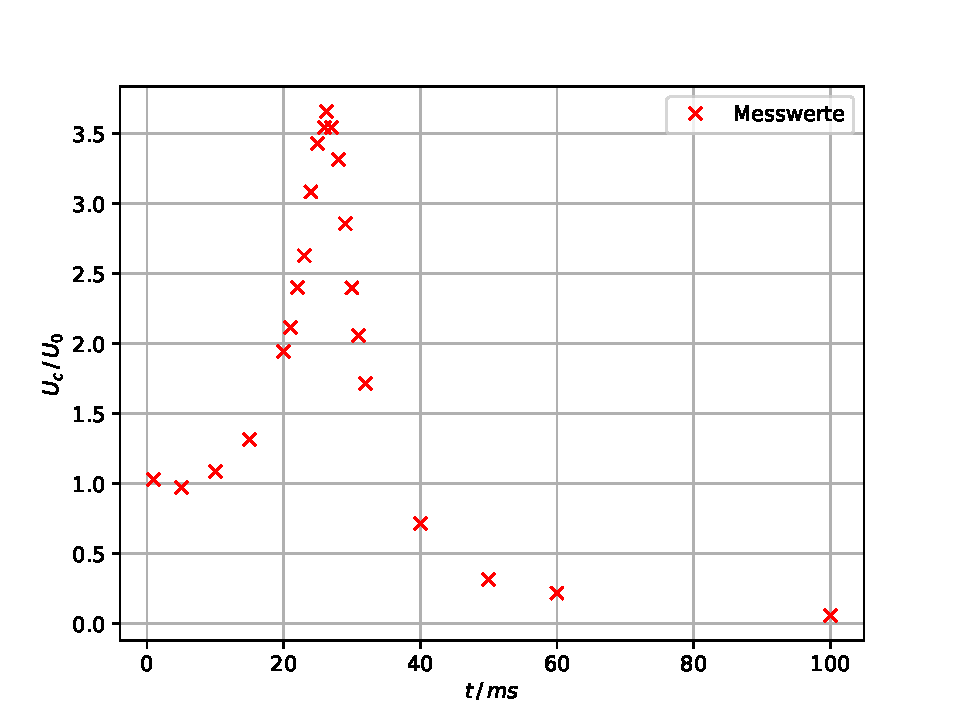
\includegraphics[width=0.6\textwidth]{content/data/plotc.pdf}
    \caption{Spannung in Abhängigkeit zur Frequenz halblogariythmisch aufgetragen.}
    \label{fig:spannung_log}
\end{figure}

\begin{figure}
    \centering
    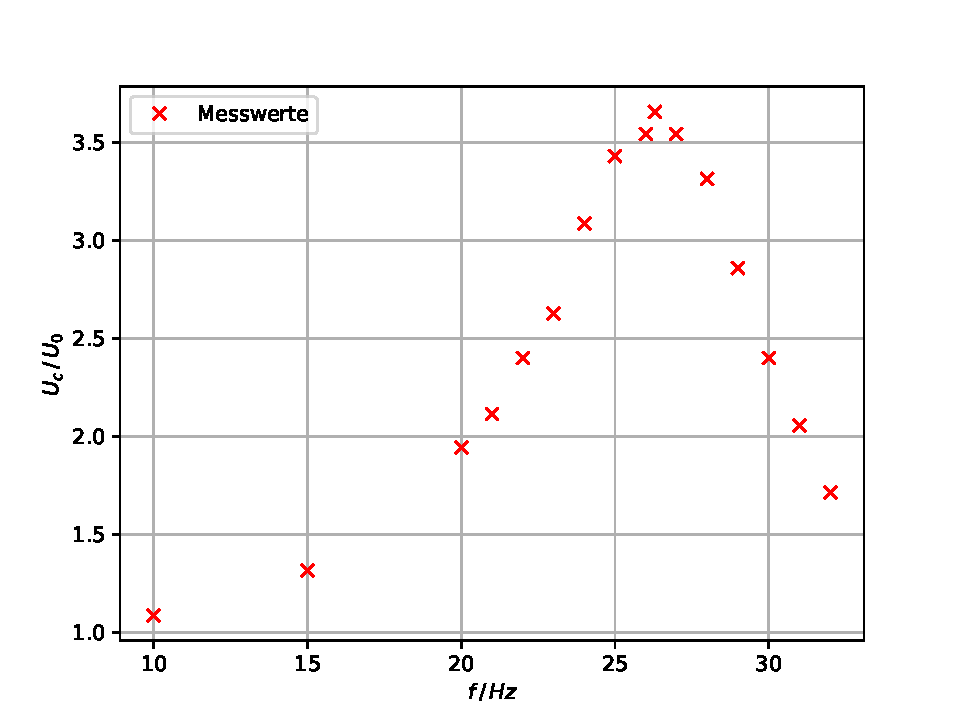
\includegraphics[width=0.6\textwidth]{content/data/plotc2.pdf}
    \caption{Spannung in Abhängigkeit zur Frequenz linear aufgetragen.}
    \label{fig:spannung_lin}
\end{figure}

\begin{figure}
    \centering
    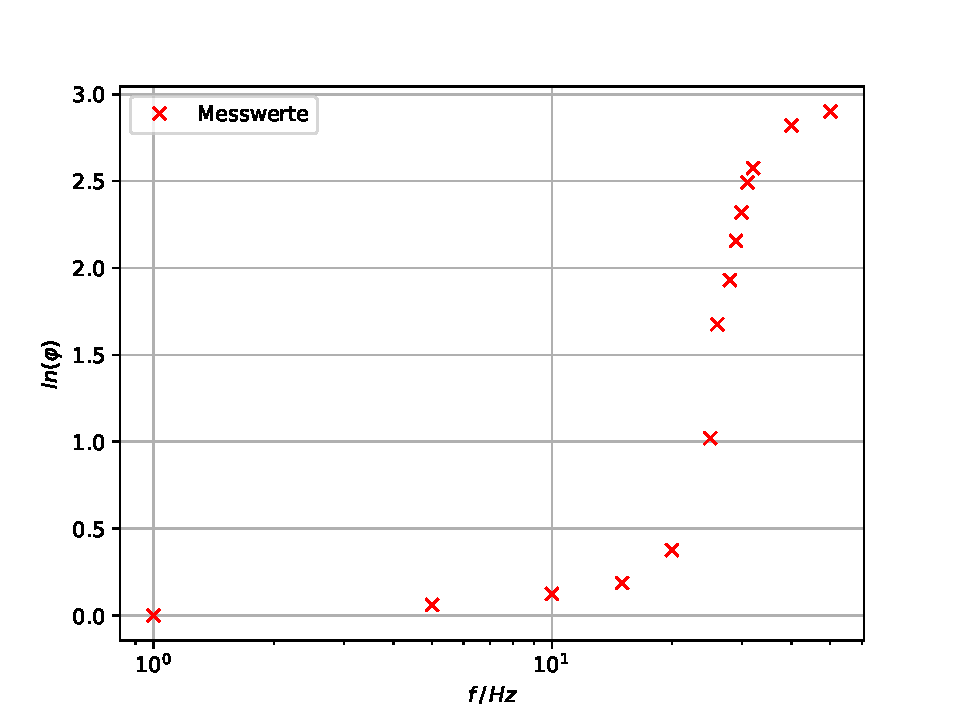
\includegraphics[width=0.6\textwidth]{content/data/plotd.pdf}
    \caption{Phasenunterschied in Abhängigkeit zur Frequenz halblogariythmisch aufgetragen.}
    \label{fig:phase_log}
\end{figure}
\begin{figure}
        \centering
        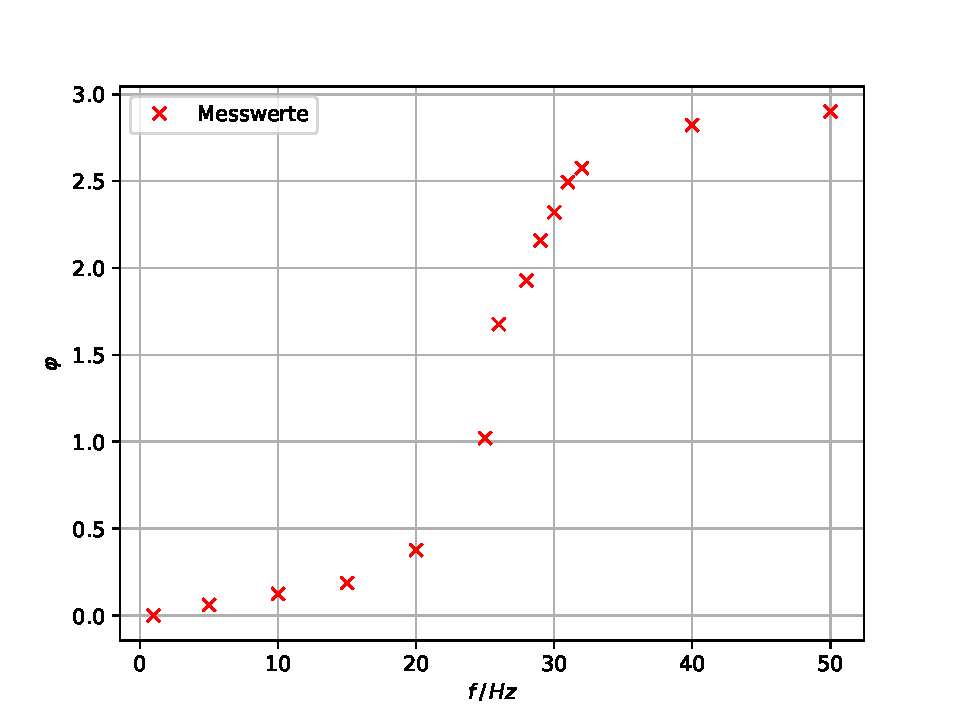
\includegraphics[width=0.6\textwidth]{content/data/plotd2.pdf}
        \caption{Phasenunterschied in Abhängigkeit zur Frequenz linear aufgetragen.} 
        \label{fig:phase_lin}
\end{figure}

\begin{table}
\centering
\caption{Der aus den Messwerten berechnete Phasenunterschied zu verschiedenen Frequenzen und die.}
\begin{tabular}[t]{cc|}
    \toprule
    $f \, / \, \si{\hertz}$ & $U \, / \, \si{\V}$\\
    \midrule
    1.0& 180    \\
    5.0& 170\\
    10.0& 190\\
    15.0& 230\\
    20.0& 340\\
    21.0& 370\\
    22.0& 420\\
    23.0& 460\\
    24.0& 540\\
    25.0& 600\\
    26.0& 620\\
    26.3& 640\\
    27.0& 620\\
    28.0& 580\\
    29.0& 500\\
    30.0& 420\\
    31.0& 360\\
    32.0& 300\\
    40.0& 125\\
    50.0& 55\\
    60.0& 38\\
    100.0& 10\\
    \bottomrule
\end{tabular}
\begin{tabular}[t]{|cccc}
    \toprule
    $f \,/\, \si{\kilo\hertz}$ & $a \,/\, \si{\milli\second}$ &  $b \,/\, \si{\milli\second}$ & $\phi$\\
    \midrule
    1& 0.0000& 1.0000& 0.0000\\
    5& 0.0020& 0.2000& 0.0628\\
    10& 0.0020& 0.1000&  0.1256\\
    15& 0.0020& 0.0670& 0.1875 \\
    20& 0.0030& 0.0500&  0.3769\\
    25& 0.0065& 0.0400&  1.0210\\
    26& 0.0096& 0.0360&  1.6755\\
    28& 0.0106& 0.0345& 1.9304 \\
    29& 0.0115& 0.0335& 2.1569\\
    30& 0.0120& 0.0325&  2.3199\\
    31& 0.0125& 0.0315 & 2.4933\\
    32& 0.0125& 0.0305& 2.5750\\
    40& 0.0110& 0.0245& 2.8210\\
    50& 0.0090& 0.0195& 2.8999\\
    100&0.0000& 0.0245& 0.0000\\
    \bottomrule
\end{tabular}
\label{tab:phase}
\end{table}
